\documentclass{beamer}
% \usepackage{geometry}
% \geometry{a4paper, portrait, margin=1in}
% \author{Lawrence Liu}
\usepackage{subcaption}
\usepackage{graphicx}
\usepackage{float}
\usepackage{amsmath}
\usepackage{pdfpages}
\newcommand{\Laplace}{\mathscr{L}}
\DeclareMathOperator{\Tr}{tr}
\setlength{\parskip}{\baselineskip}%
\setlength{\parindent}{0pt}%
\usepackage{xcolor}
\usepackage{listings}
\definecolor{backcolour}{rgb}{0.95,0.95,0.92}
\usepackage{amssymb}
\lstdefinestyle{mystyle}{
    backgroundcolor=\color{backcolour}}
\lstset{style=mystyle}

\title{A Kernel Density Based Approach to Portfolio Optimization}
\author{Lawrence Liu}
\date{June 2023}

\begin{document}
\frame{\titlepage}
\begin{frame}
\frametitle{Introduction: Problem Statement}

    \textbf{Goal: Portfolio Optimization}, given a set of $m$ stocks, find the allocation of funds to each stock that maximizes the sharpe ratio:
    \begin{equation}
        \text{Sharpe Ratio} = \frac{\mu_r}{\sigma_r}\sqrt{252}
    \end{equation}
    Where $\mu_r$ is the expected day to day return of the portfolio, $\sigma_r$ is the standard deviation of the day to day returns of the portfolio.\\
    \textbf{Constraints:} The sum of the weights must be 1, and each weight must be between 0 and 1. And we must use a buy and hold strategy, i.e. we cannot change the amount of money allocated to each stock over time.
% \end{itemize}
\end{frame}

\begin{frame}
\frametitle{Introduction: Modern Portfolio Theory}
    \begin{itemize}
        \item Previous approach: \textbf{Markowitz Portfolio Optimization}
        \item Assume the returns of each stock are normally distributed, ie if the day to day return of all the stocks $r$ distributed as $r \sim \mathcal{N}(\mu, \Sigma)$
        \item Then the expected return of the portfolio is $\mu_r = w^T\mu$ and the variance of the portfolio is $\sigma_r^2 = w^T\Sigma w$
        \begin{equation}
            \begin{aligned}
                & \underset{w}{\text{maximize}}
                & & \frac{w^T\mu}{\sqrt{w^T\Sigma w}} \\
                & \text{subject to}
                & & 1^Tw_i = 1 \\
                & & & w_i \geq 0 \quad \forall i \in \{1, \dots, n\}
            \end{aligned}
        \end{equation}
    \end{itemize}
\end{frame}
\begin{frame}
\frametitle{Introduction: Solution to Fractional Programming}
    To solve that equation we do the following.\\
    We introduce a dummy variable $y=\alpha w$, where $\alpha=1^T y$. Then we can reformulate the problem as:
    \begin{equation}
        \begin{aligned}
            & \underset{y}{\text{minimize}}
            & & y^T\Sigma y\\
            & \text{subject to}
            & & \mu^Ty = 1 \\
            & & & y_i \geq 0 \quad \forall i \in \{1, \dots, n\}
        \end{aligned}
    \end{equation}
    This is a convex problem and can be solved using a quadratic programming solver. Then we have $w = \frac{y}{1^Ty}= \frac{y}{\alpha}$.
\end{frame}
\begin{frame}
    \frametitle{Introdcution: Problems with Modern Portfolio Theory}
    MPT makes the following assumptions:
    \begin{itemize}
        \item The returns of stocks are not normally distributed
        \item The returns of the stocks are stationary with time
    \end{itemize}
    Today we will show that the first assumption is not true and propose a new method that is not reliant on the first assumption
\end{frame}
\begin{frame}
    \frametitle{Methods: Data}
    \begin{itemize}
        \item We scraped the data from Yahoo Finance using the \texttt{yfinance} python package for all the stocks in the S\&P 500 
        \item We used the data from 2010-01-01 to 2020-01-01
        \item Because some tickers were not trading for the entire time period, we only used the tickers that were trading for the entire time period, thus we had 428 companies in our dataset.
        \item We separated the data into the first 8 years being train and the last 2 years being test we used to evaluate our model on.
    \end{itemize}
\end{frame}
\begin{frame}
    \frametitle{Non-Normality of Stock Returns}
    \begin{itemize}
    \item Perform a Kolmogorov-Smirnov Test on the day to day changes in stock price for each ticker
    \item At Significance $0.001$, we can reject the Null Hypothesis that the day to day changes in stock price are distributed 
        according a fitted Normal Distribution
    \item Also plotted out distribution of day to day change of the S\&P 500 stock price and fitted normal
    \begin{figure}[H]
        \centering
        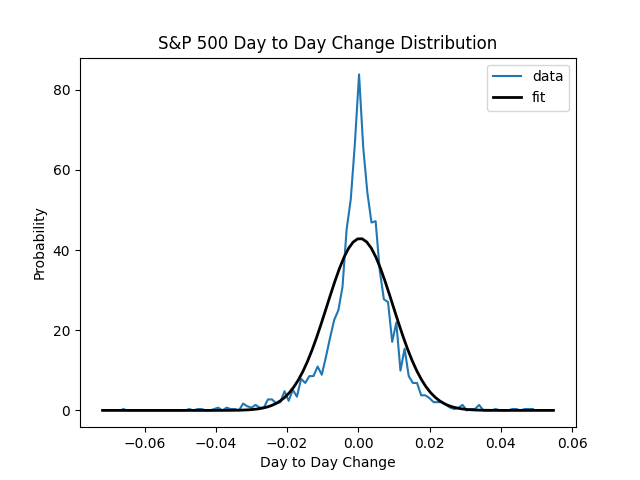
\includegraphics[width=0.6\textwidth]{../day_to_day_change.png}
        % \caption{Histogram of the returns of all the stocks}
        % \label{fig:returns_hist}
    \end{figure}
\end{itemize}
\end{frame}
\begin{frame}
    \frametitle{Our Method}
    Our method is twofold:
    \begin{itemize}
        \item A nonparametric Kernel Density Estimation (KDE) to obtain a more accurate estimate for the portfolio variance
        \item A spectral clustering based method to break the problem into smaller sectors to first find an optimal portfolio for
    \end{itemize}
\end{frame}
\begin{frame}
    \frametitle{Kernel Desnity Estimation}
    We estimate the multivariate distribution of all day to day changes of all the stocks $x$ in our dataset using a kernel density estimation.
    \begin{equation}
        \hat{f}_{\Sigma}(x) = \frac{1}{n} \sum_{i=1}^n K_{\Sigma}(x-x_i')
    \end{equation}
    Where $x_i'$ is the $i$th training point. 
    In our case $x_i'$ is a $m$ dimensional vector representing the daily change for each of the $m$ stocks in our dataset. We use 
    a Gaussian Kernel 
    \begin{equation}
        K_{\Sigma}(x) = \frac{1}{\sqrt{(2\pi)^d|\Sigma|}}\exp\left(-\frac{1}{2}x^T\Sigma^{-1}x\right)
    \end{equation}
\end{frame}
\begin{frame}
    \frametitle{Kernel Density Estimation: Optimizing $\Sigma$}
    We optimize $\Sigma$ by splitting the training data into a training and validation set.
     We then optimize $\Sigma$ by minimizing the negative log likelihood of the validation set.
    \begin{equation}
        \mathcal{L}(x_1,\dots,x_k) = -\sum_{i=1}^k \log(\hat{f}_{\Sigma}(x_i))
    \end{equation}
    Where $x_1,\dots,x_k$ are the validation datapoints.\\
    Because $\Sigma$ is positive semidefinite, we use Cholesky factorization $\Sigma = R^TR$ to optimize $R$ instead.
    \begin{align*}
        \frac{\partial}{\partial R}\mathcal{L}(x_1,\dots,x_k) \approx &\sum_{i=1}^k \frac{1}{\hat{f}(x_i)} \sum_{j=1}^n K_{\theta}(x_i-x_j')\left(R^{-T} - \right.\\
        &\left.\Sigma^{-1}(x_i-x_j')(x_i-x_j')^T R^{-1}\right)
    \end{align*}
\end{frame}
\begin{frame}
    \frametitle{Kernel Density Estimation: A More Accuracte Estimate of Portfolio Variance}
    From some math we get that the portfolio variance is given by 
    \begin{multline}
        \mathbb{E}[(w^Tx)^2]-\mathbb{E}^2[w^Tx] = w^T\left(\Sigma +  \frac{1}{n}\sum_{i=1}^nx_i'x_i'^T - \right.
        \\ \left.\left(\frac{1}{n} \sum_{i=1}^nx_i'\right)\left(\frac{1}{n} \sum_{i=1}^nx_i'\right)^T\right)w
    \end{multline}
    %     \mathbb{E}[(w^Tx)^2]-\mathbb{E}^2[w^Tx] = w^T\left(\Sigma +  \frac{1}{n}\sum_{i=1}^nx_i'x_i'^T - \left(\frac{1}{n} \sum_{i=1}^nx_i'\right)\left(\frac{1}{n} \sum_{i=1}^nx_i'\right)^T\right)w
    % \end{equation}
    Therefore we can isolate the part between the $w^T$ and $w$ as the covariance matrix of the kernel density estimate.
\end{frame}
\begin{frame}
    \frametitle{Spectral Clustering}
    \begin{itemize}
        \item To identify each sector, we would want stocks that are highly correlated with each other to be in the same sector
        \item Thus we use spectral clustering, with the adjacency matrix being the negative of the correlation matrix of the stocks
        \item To identify the number of sectors, we use the eigengap heuristic, but we limit the number of sectors to be between 5 and 50
    \end{itemize}
\end{frame}
\begin{frame}
    \frametitle{Spectral Clustering Results: Eigengap}
    \begin{figure}[H]
        \centering
        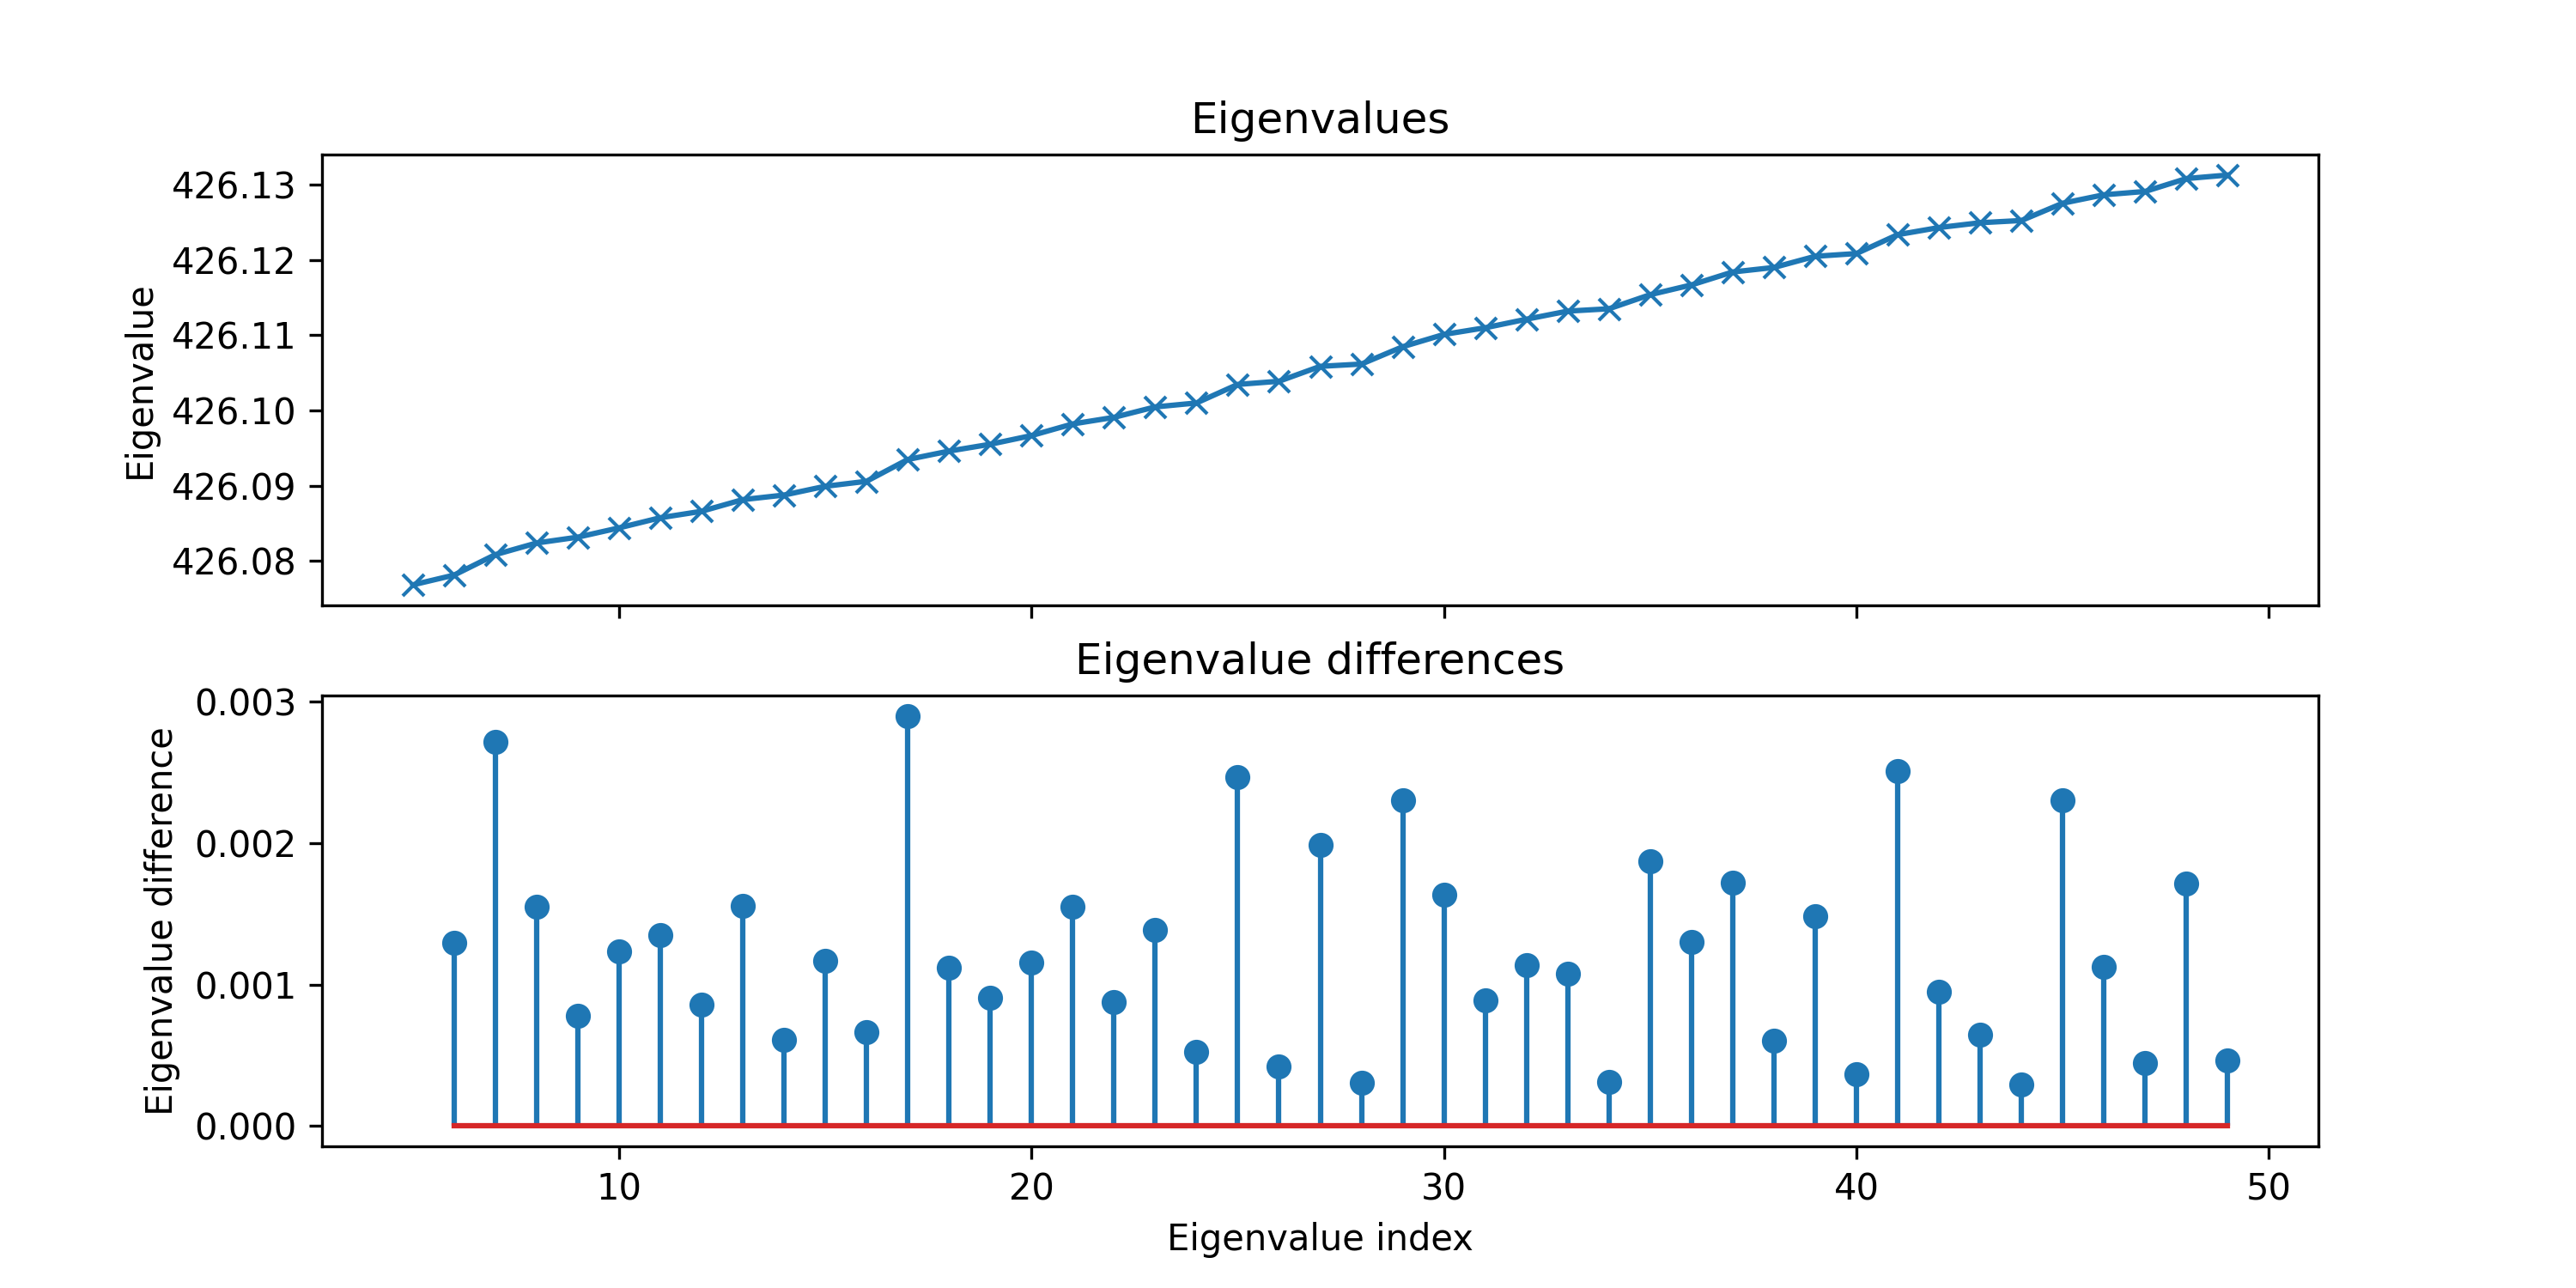
\includegraphics[width=0.9\textwidth]{../eigenvalues.png}
        % \caption{Histogram of the returns of all the stocks}
        % \label{fig:returns_hist}
    \end{figure}
    We used 17 sectors for our model    
\end{frame}
\begin{frame}
    \frametitle{Spectral Clustering Results: Correlation Matrix}
    \begin{figure}[H]
        \centering
        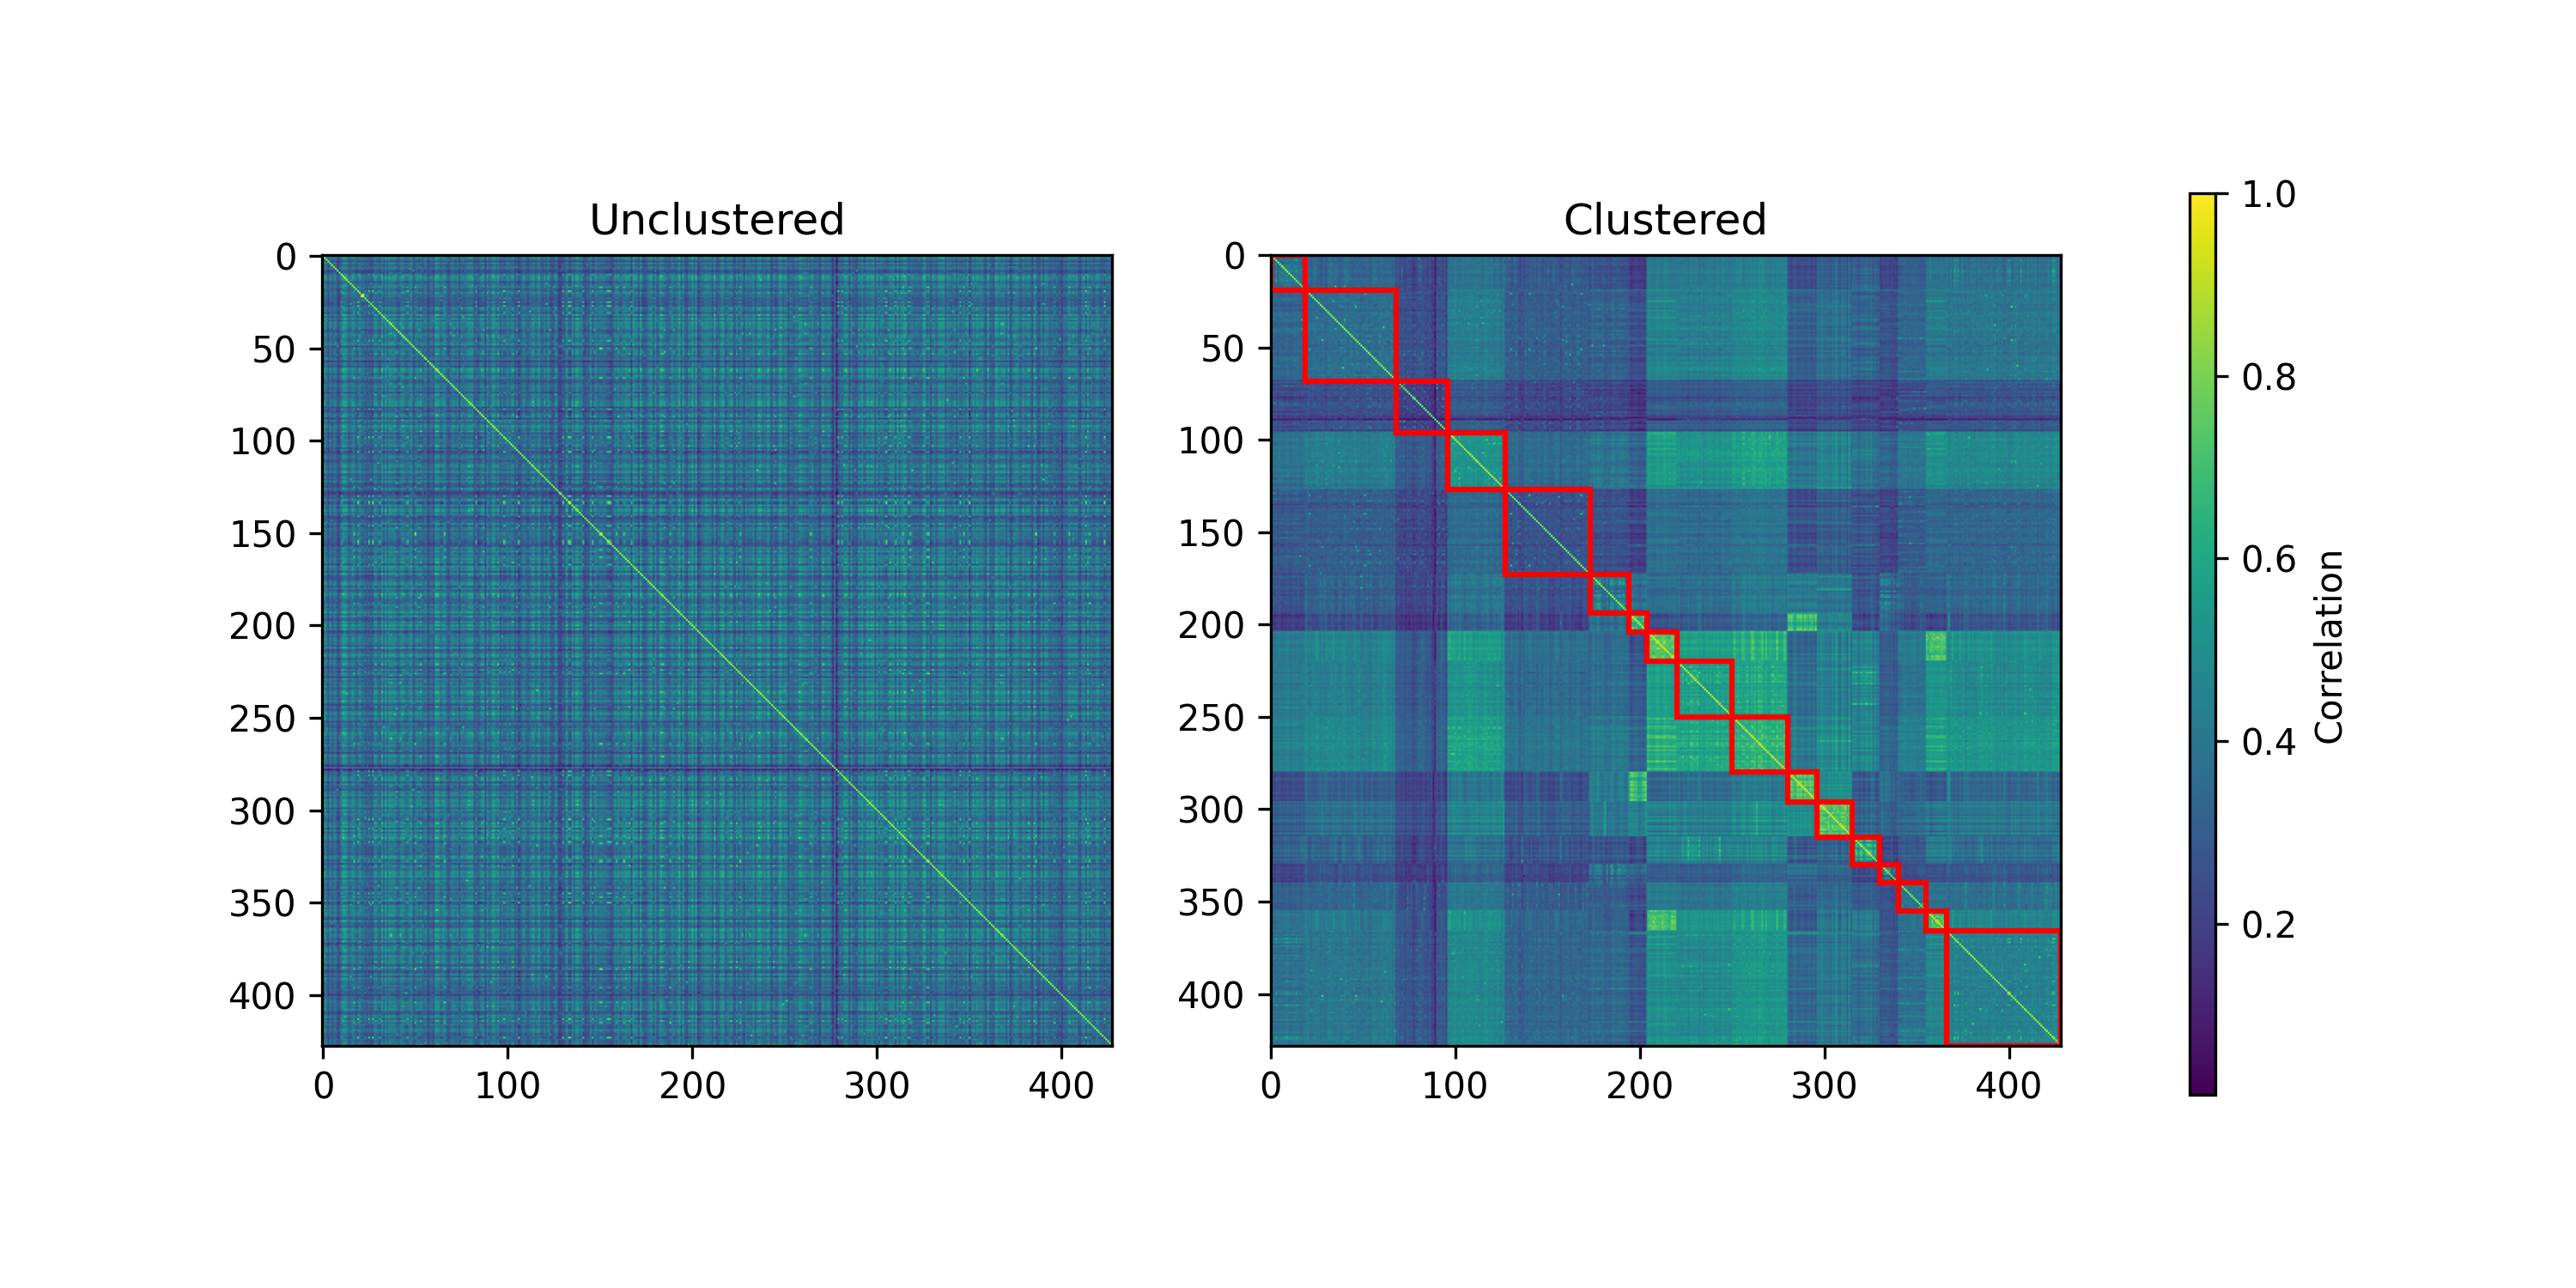
\includegraphics[width=\linewidth]{../clustered_corr.png}
        % \caption{Histogram of the returns of all the stocks}
        % \label{fig:returns_hist}
    \end{figure}
\end{frame}
\begin{frame}
    \frametitle{Spectral Clustering Results: Individual Sectors}
    \begin{table}
        \centering
        \begin{tabular}{|c|c|}
            \hline 
            Ticker & Company \\
            \hline
            AMP & Ameriprise Financial, Inc. \\
            BK & The Bank of New York Mellon Corporation \\
            C & Citigroup Inc. \\
            FITB & Fifth Third Bancorp \\
            JPM & JPMorgan Chase \& Co. \\
            LNC & Lincoln National Corporation \\
            MET & MetLife, Inc. \\
            NTRS & Northern Trust Corporation \\
            PNC & The PNC Financial Services Group, Inc. \\
            PRU & Prudential Financial, Inc. \\
            RJF & Raymond James Financial, Inc. \\
            STT & State Street Corporation \\
            HIG & The Hartford Financial Services Group, Inc. \\
            TFC & Truist Financial Corporation \\
            USB & U.S. Bancorp \\
            WFC & Wells Fargo \& Company \\
            \hline
        \end{tabular}
        % \caption{The tickers in cluster 7}
        \label{tab:clusters7}
    \end{table}
\end{frame}
\begin{frame}
    \frametitle{Overall Results}
    \begin{table}[H]
        \centering
        \begin{tabular}{|p{0.45\linewidth}|p{0.15\linewidth}|p{0.15\linewidth}|}
            \hline
            Method & Sharpe Ratio (train) & Sharpe Ratio (test)\\
            \hline
            S\&P 500 & 0.804 & 0.709 \\
            Markowitz & 2.266 & 1.199 \\
            KDE & 1.201 & 0.920 \\
            Spectral Clustering + KDE & 1.969 & 1.424\\
            \hline
        \end{tabular}
        % \caption{Sharpe Ratios for each method}
        \label{tab:sharpe_ratios}
    \end{table}
    \begin{table}[H]
        \centering
        \begin{tabular}{|c|c|c|}
            \hline
            Method & YOY (train) & YOY (test)\\
            \hline
            S\&P 500 & 11.352 \% & 9.947\% \\
            Markowitz & 37.699\% & 15.969\% \\
            KDE & 19.362\% & 12.743\% \\
            Spectral Clustering + KDE & 25.246\% & 17.398\%\\
            \hline
        \end{tabular}
        % \caption{Year over Year Returns for each method}
        \label{tab:YoY_returns}
    \end{table}
\end{frame}
\begin{frame}
    \frametitle{Discussion and Conclusion}
    \begin{itemize}
        \item Spectral Clustering is able to cluster the correlation matrix to be more block diagonal, and it is able to identify related stocks into one sector.
        \item Our model of Spectral Clustering+KDE outperforms both the S\&P 500 and the Markowitz model on the test dataset.
        \item Pure KDE Model is not able to outperform the Markowitz model on the test dataset. We believe this is because of the curse of dimensionality.
        \item Intrestingly,the Markowitz model performs better than KDE with and without Spectral Clustering on the training dataset, but not on the test dataset.
    \end{itemize}
\end{frame}
\begin{frame}
    \frametitle{Future Directions}
    \begin{itemize}
        \item Experiment with different kernels for the KDE, such as Multivariate T distribution
        \item Experiment with more powerful optimization algorithms such as Adam or SGD with Momentum
        \item Experiment with improving runtime of the KDE with multiprocessing/GPU acceleration
        \item Experiment with a different heuristic for choosing the number of sectors
        \item Find a way to deal with the non-stationarity of the data
    \end{itemize}
\end{frame}

\end{document}